\documentclass{article}
\usepackage[final]{listings}
\usepackage{color}
\usepackage{float}
\usepackage{xcolor}

\usepackage{caption}
\DeclareCaptionFont{white}{\color{white}}
\DeclareCaptionFormat{listing}{\colorbox{gray}{\parbox{\textwidth}{#1#2#3}}}
\captionsetup[lstlisting]{format=listing,labelfont=white,textfont=white}

\usepackage{graphicx}
\usepackage{enumerate}
\usepackage[utf8]{inputenc}
\usepackage[spanish]{babel}
\usepackage[T1]{fontenc}

\begin{document}
\begin{center}
{\LARGE \textbf{
Teor\'ia de lenguajes, aut\'omatas y compiladores\\}
Trabajo pr\'actico 2\\
Generador de Analizador Sint\'actico Descendente con Retroceso (ASDR)\\
ITBA\\
}
\end{center}

\vspace{12cm}
\begin{flushright}

 \textbf{Conrado E. F. Mader Blanco} - Legajo 51270\\
 \textbf{Tom\'as Alfredo Mehdi} - Legajo 51014\\
 \textbf{Federico Ramundo} - Legajo 51596 
 
 \end{flushright}
\newpage
\tableofcontents
\newpage
\section{Objetivo}
El trabajo consiste en programar en C un Generador de Analizador Sint\'actico Descendente con Retroce- so(ASDR). Dada una gram\'atica libre de contexto, sin recursividad a izquierda, el programa deber\'a generar un ASDR que estar\'a escrito en lenguaje C.(ASDR.c). El ASDR pod\'ra luego recibir una cadena de entrada y determinar si pertenece o no al lenguaje generado por la gram\'atica, mostrando adem\'as la derivaci\'on que llev\'o a dicha cadena.

\section{Funcionamiento del programa}
El generador recibe como entrada un archivo de extensi\'on .gr, donde est?a la especificaci\'on de una sola gram\'atica que se asume libre de contexto y sin recursividad a izquierda. La sintaxis de ejecuci\'on del generador es:
\begin{center}
genASDR nombrearchivogramatica
\end{center}
El generador obtiene como salida un archivo ASDR.c que ser?a el c\'odigo fuente del Analizador Sint\'actico Descendente con Retroceso implementado a trav\'es de procedimientos.\\

El ADSR tiene una funci\'on principal , una funci\'on por cada no terminal de la gram\'atica y una funci\'on para procesar la cadena de entrada.\\
Se utiliz\'o la heur\'istica siguiente: mientras el m\'etodo intenta diferentes derivaciones, si el conjunto de hojas del \'arbol es mayor a la longitud de la cadena a analizar entonces se aplica el retroceso.

\section{Estructura de las gram\'aticas}
Un archivo de gram\'atica (.gr) es un archivo en el que se especifican las gram\'aticas de la siguiente forma: 
\begin{center}
NombreDeLaGramatica = ( {SimbolosNoTerminales}, {SimbolosTerminales}, SimboloInicial, {Producciones})
\end{center}
En esta estructura se tienen las siguientes consideraciones:
\begin{itemize}
\item Los SimbolosNoTerminales son letras en mayu\'scula separadas por comas.
\item Los SimbolosTerminales son letras en minu\'scula separadas por comas.
\item Para el s\'imbolo lambda se usa el caracter \textbackslash (barra invertida).
\item Los caracteres del archivo pueden (o no) estar separados por espacios, tabuladores o fines de linea.
\item Se recibe una sola gram\'atica por archivo.
\item El nombre de la gram\'atica empieza por una letra.(despu\'es puede seguir cualquier s\'imbolo, sin espacios.
\end{itemize}

\section{Funcionamiento del ASDR}
El analizador recibe como entrada una palabra que podr\'ia pertenecer al lenguaje es decir, una cadena formada s\'olo por letras min\'usculas. La sintaxis de ejecuci\'on del analizador es: 
\begin{center}
ASDR palabra
\end{center}
El programa ASDR devuelve '$palabra$ doesn't belong.' si la cadena no pertenece o '$palabra$ belongs' y a continuaci\'on el conjunto de producciones que dieron lugar a dicha palabra.

\section{Consideraciones realizadas}
Para ejecutar el \textit{parsing} de la entrada de archivos se utiliz\'o LEX tal y como hicimos con el trabajo anterior.\\
Para realizar el funcionamiento del trabajo se utiliz\'o el algoritmo provisto por la c\'atedra en la teor\'ia. Implementamos el algoritmo provisto y adaptamos las estructuras definidas por el trabajo anterior. Antes, al evaluar s\'olo gram\'aticas regulares guard\'abamos como mucho dos caracteres en la parte derecha de las producciones. Ahora al ser libres de contexto pueden venir varios caracteres.

\section{Dise\~no y desarrollo}
\subsection{An\'alisis de la gram\'atica}
Tal y como se mencion\'o anteriormente, para controlar que el archivo de entrada sea correcto nos proveemos de la herramienta LEX. A su vez, la utilizamos para armar la estructura de la gram\'atica en memoria.\\
Una vez obtenida la gram\'atica se procede a generar el archivo compilabre $ASDR.c$. Para ello se imprime en un archivo lineas de c\'odigo C, en base a la estructura de la gram\'atica.
\subsection{Procesamiento de cadenas}

Para procesar las cadenas se tiene una funci\'on que retorna un booleano que procesa una cadena, bas\'andose en el algoritmo visto en clase: Se genera una funci\'on por cada s\'imbolo no terminal y se va consumiendo la cadena a medida que se avanza por las funciones. Si se produce un error entonces no se acepta esa cadena. Si por otro lado se llega al final de la cadena y las funciones terminan positivamente, se acepta la cadena.\\
Se guarda, adem\'as, las producciones utilizadas para luego poder imprimirlas e indicar al usuario cual es el camino a seguir para obtener dicha cadena.

\section{Dificultades encontradas}

En general podemos decir que este trabajo nos pareci\'o m\'as f\'acil que el anterior, dado que ya nos defend\'iamos mejor con LEX. Adem\'as, el m\'etodo de an\'alisis descendente lo ten\'iamos fresco del parcial que dimos hace s\'olo unas pocas semanas, y nos acord\'abamos bastante del procedimiento a seguir.\\
El lenguaje C no genera problemas dado que ya estamos acostumbrados a programar con \'el desde hace 3 a\~nos de carrera.

\section{Futuras extensiones}
Una posible extensi\'on podr\'ia ser desarrollar un analizador sint\'ctico ascendente. Para ello se tendr\'ia que cambiar el funcionaminto de varias funciones para seguir el algoritmo correspondiente con los analizadores ascendentes. Resultar\'ia interesante que el usuario pudiese elegir a la hora de ingresar una gram\'atica si la desea analizar ascendente o descenentemente.\\
Otra posible extensi\'on podr\'ia ser que el programa mantenga un log de las producciones que fue probando y las reducciones que realiz\'o, para darse una idea de si la heur\'istica utilizada es buena o si al analizador le est\'a costando mucho llegar a la conclusi\'on.\\


\section{Ejemplo de uso}
Dada la gram\'atica:
\begin{center}
G1 = ({A, B, C}, {a, b, c},A, {A -> aBC|cB, B -> aA|b, C -> c|\textbackslash})
\end{center}
Se ejecuta el comando \textit{./bin/genASDR ./gr/ejemplo.gr} y se obtiene un archivo llamado ASDR.c.\\
A continuaci\'on se compila con la linea \textit{gcc -o gram1 ASDR.c} y se ejecuta pas\'andole una cadena, tal y como se ve en la \ref{fig:ejemplo}.
 
\begin{figure}[H]
\centering
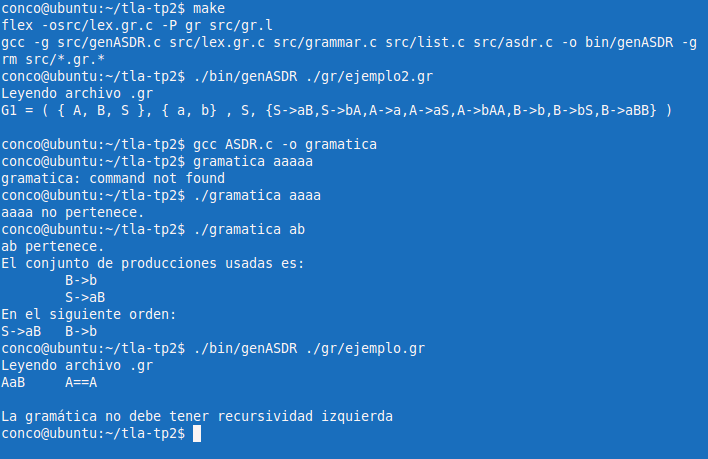
\includegraphics[scale=1]{./fotos/ejemplo.png}
\caption{ Ejemplo de uso}
\label{fig:ejemplo}
\end{figure}
\end{document}
